% * Provide Electricity to remote areas. no infrastructure needed. renewable and sustainable. no running cost once installed. easy to maintain.

% * Enables access to basic modern technology: phones, computers radios and medical equipment.

% * Cost is the main driving factor for renewable energy. remote areas RE is cheap, because of no infrastructure real infrastructure needed. However is expensive for industrial areas, or major city's 

% The introduction of low-power electronics brings a new set of luxuries and increased quality of living to the population. for example tv, radios, mobile phones and medical equipment. requires low voltage DC electricity (5-12V). contain battery's, day long. therefore, only intermittant power is needed to charge devices. higher bust power required for charging or medical devices -> reserve power also helpful to on cloudy days.


% requirments:

%  must be cheap. for remote areas, this means no infrastructure. aka no grid and no fuel. 

%  sustainable best option, no running cost once installed, easy to maintain. no need to travel to get fuel which is expensive.



% * near equator with high solar radiation, solar power is a good option.



Introducing low-power electronics brings a new set of luxuries and increased quality of living to the population, for example, tv, radios, mobile phones and medical equipment. These applications require low-voltage DC electricity (5v-12v). Some of these devices contain batteries, which can last a day long. While intermittent power is adequate for these devices, a more sophisticated system might require higher burst power for fast charging or medical devices.


A low price is the primary driving factor for implementing new electrical systems to power such devices. Given the developing status and lack of infrastructure, renewable and sustainable power is the best option. The cost of extending the grid makes it unfeasible, and combined with limited accessibility meaning fuel is expensive to transport, the system must be self-sufficient.

The country has high solar radiation and PV potential because it is near the equator, making solar power a good option. The relative humidity in the rainforest regions is high, hence more clouds leading to less solar radiation. However, the country is still a good candidate for solar power, as the average daily solar radiation is around 5.5kWh/m2 \cite{Aly2017Dec}. A 20\% efficacy 1x1m solar panel would produce, on average 1.1 kWh daily, based on the average daily energy consumption of 274Wh would power a rondavel of 3 people. 

\begin{figure}[!ht]
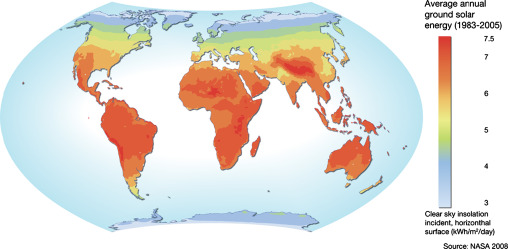
\includegraphics[width=0.8\textwidth]{IMG/pvp.jpg}
\caption{Average daily solar radiation in Tanzania \cite{Aly2017Dec}}
\label{fig:4_Review_2}
\end{figure}

Hence small isolated solar panels are helping to bring Tanzania into the modern world. They provide the cheapest form of electricity to remote places. They require minimal maintenance, hence no reliance on other civilisations. They are minimally invasive and can be installed on the roof of a rondavel. They are also sustainable, as they require no fuel to run and no running cost once installed.